\chapter{結果與討論}
%\renewcommand{\baselinestretch}{10.0} %設定行距
\section{展示案例研究的結果}

這次使用了車門鎖的機構來當案例,由圖\ref{4.0}可知,主要的開門結構主要由5個零件來組成(圖\ref{4.1} - 圖\ref{4.10}),在本次的案例中,會使用Solid Edge來繪製零件圖並組合,再來簡單解說開門時結構的運作模式。\\
\begin{figure}[hbt!]
\begin{center}
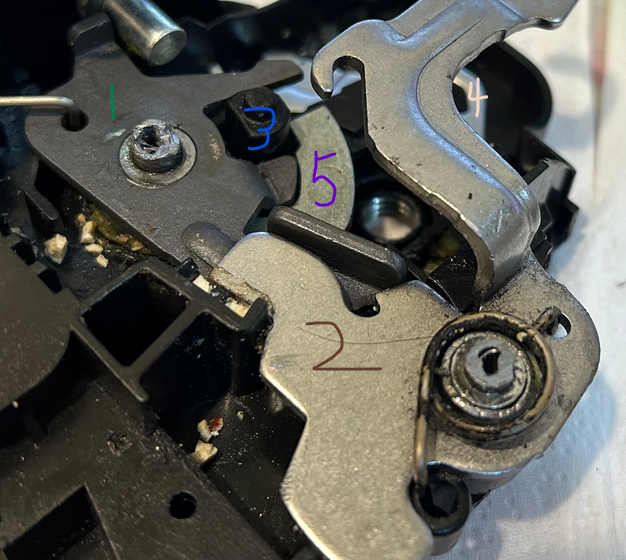
\includegraphics[width=12cm]{現實中控鎖0}
\caption{\Large 車門結構零件}\label{4.0}
\end{center}
\end{figure}
\\
\begin{figure}[hbt!]
\begin{center}
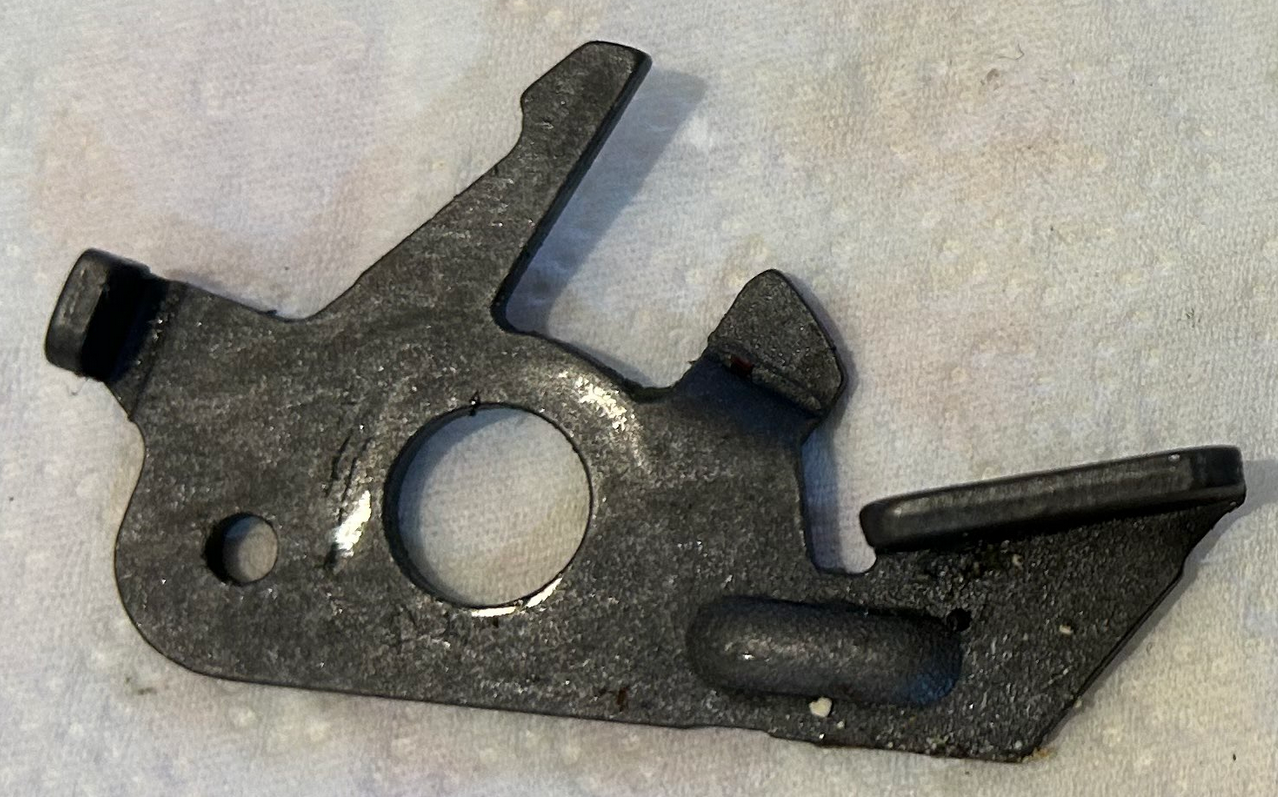
\includegraphics[width=12cm]{現實中控鎖1}
\caption{\Large 車門鎖結構零件}\label{4.1}
\end{center}
\end{figure}
\\
\begin{figure}[hbt!]
\begin{center}
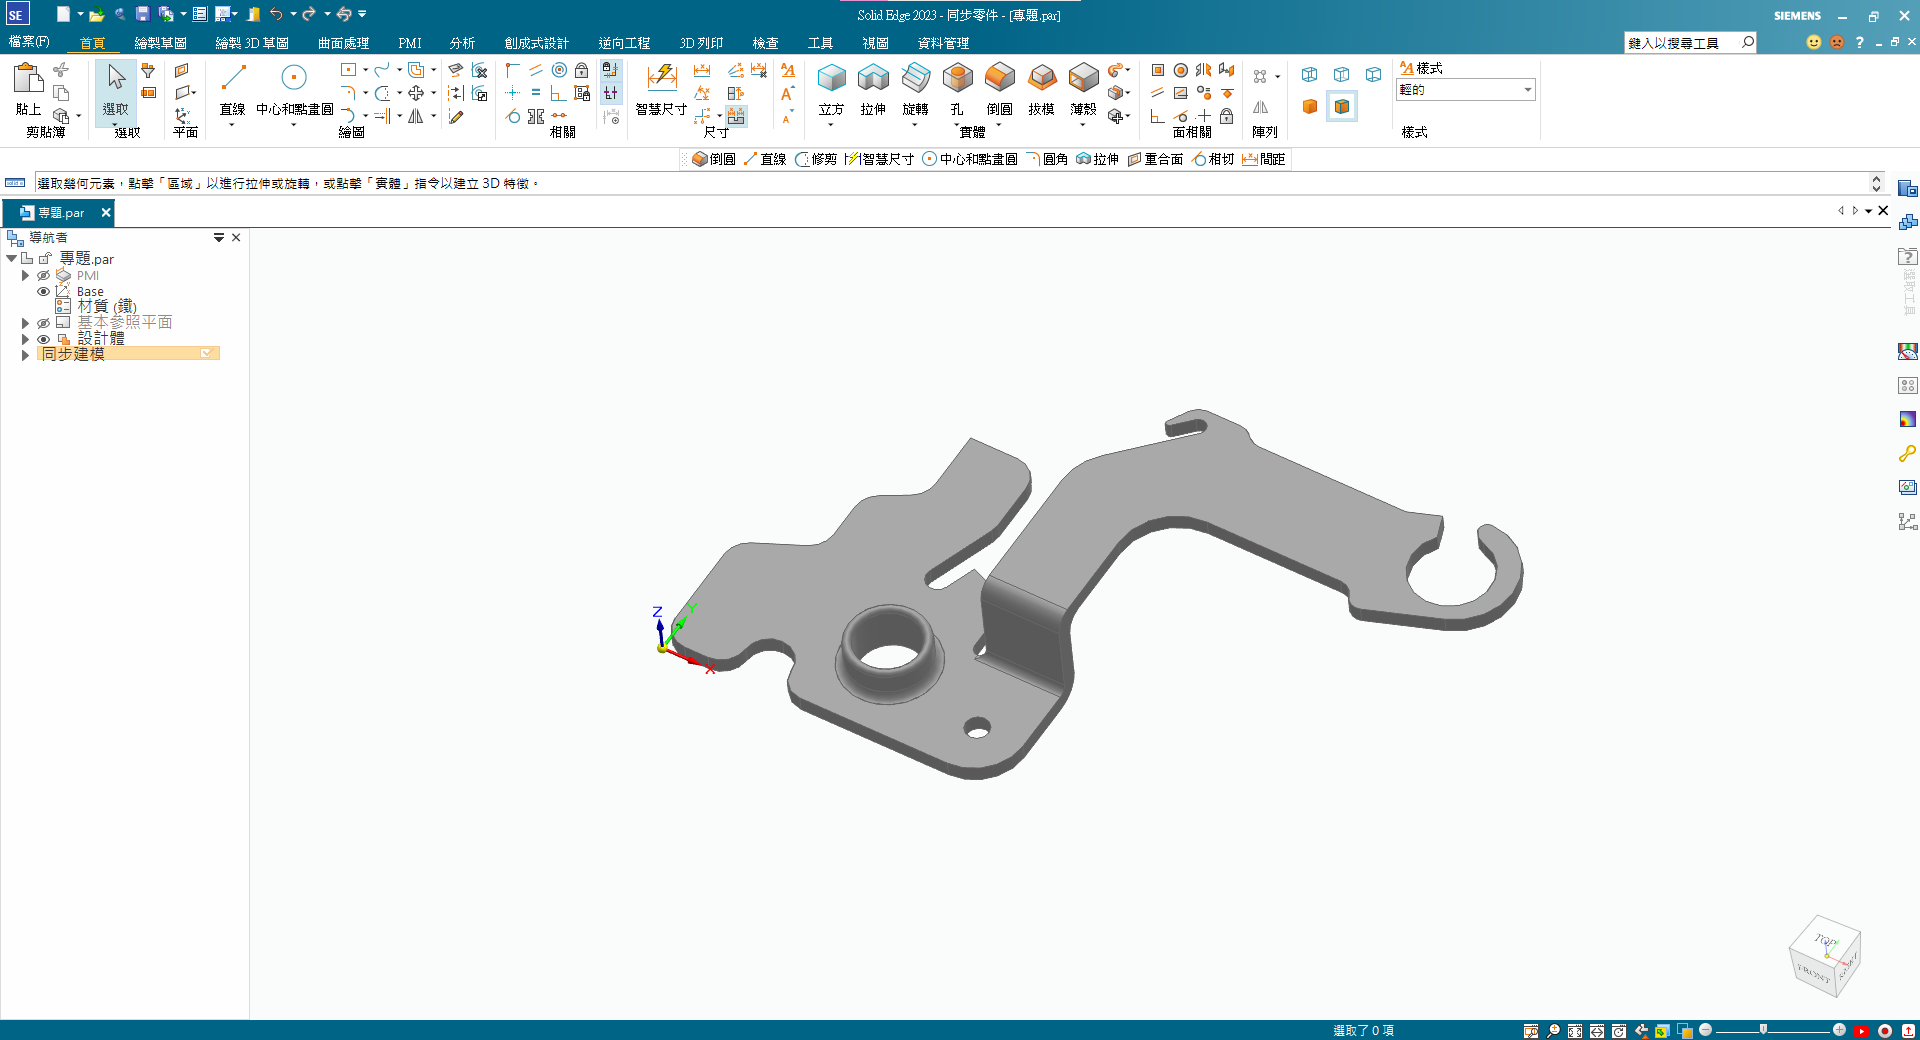
\includegraphics[width=10cm]{中控鎖1}
\caption{\Large 車門鎖零件模型}\label{4.6}
\end{center}
\end{figure}
\\
\begin{figure}[hbt!]
\begin{center}
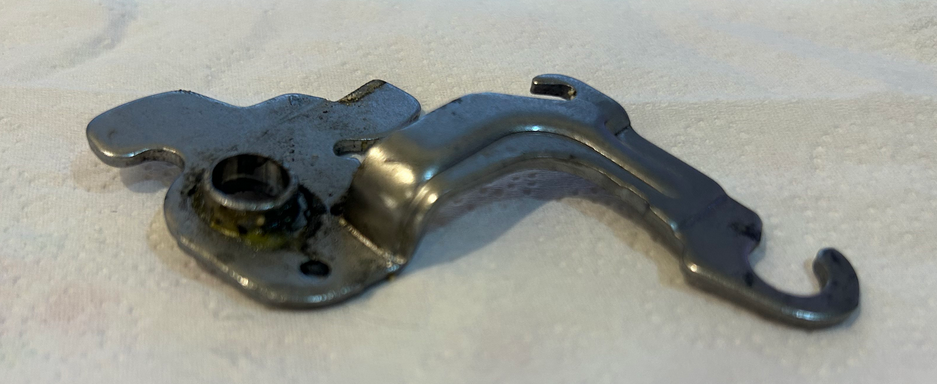
\includegraphics[width=12cm]{現實中控鎖2}
\caption{\Large 車門鎖結構零件}\label{4.2}
\end{center}
\end{figure}
\\
\begin{figure}[hbt!]
\begin{center}
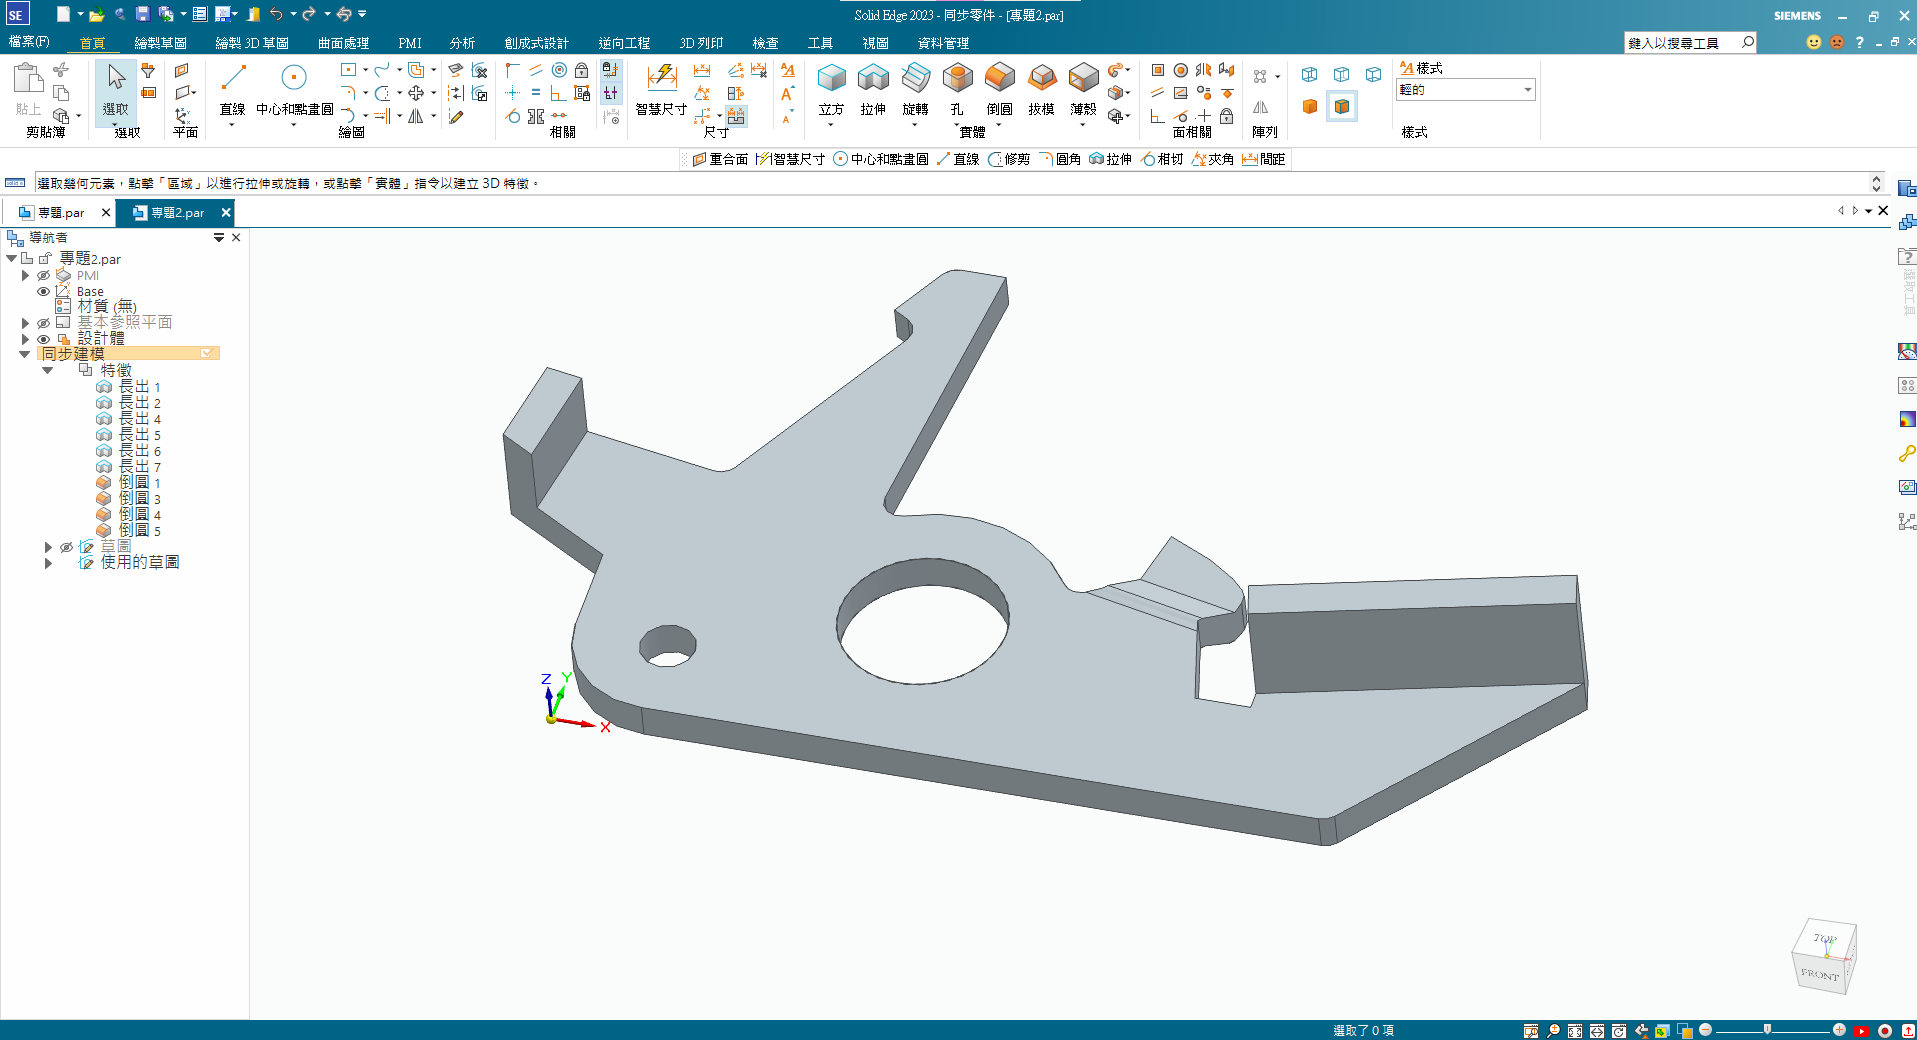
\includegraphics[width=10cm]{中控鎖2}
\caption{\Large 車門鎖零件模型}\label{4.7}
\end{center}
\end{figure}
\\
\begin{figure}[hbt!]
\begin{center}
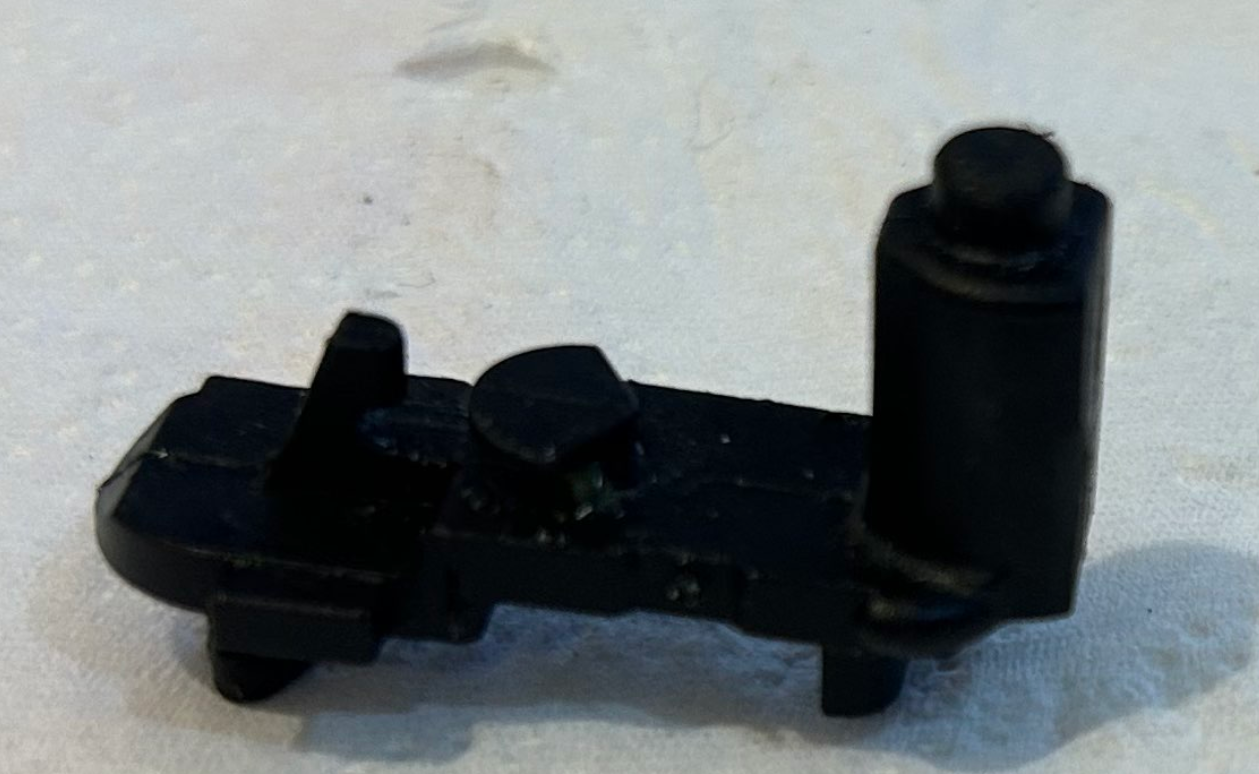
\includegraphics[width=12cm]{現實中控鎖3}
\caption{\Large 車門鎖結構零件}\label{4.3}
\end{center}
\end{figure}
\\
\begin{figure}[hbt!]
\begin{center}
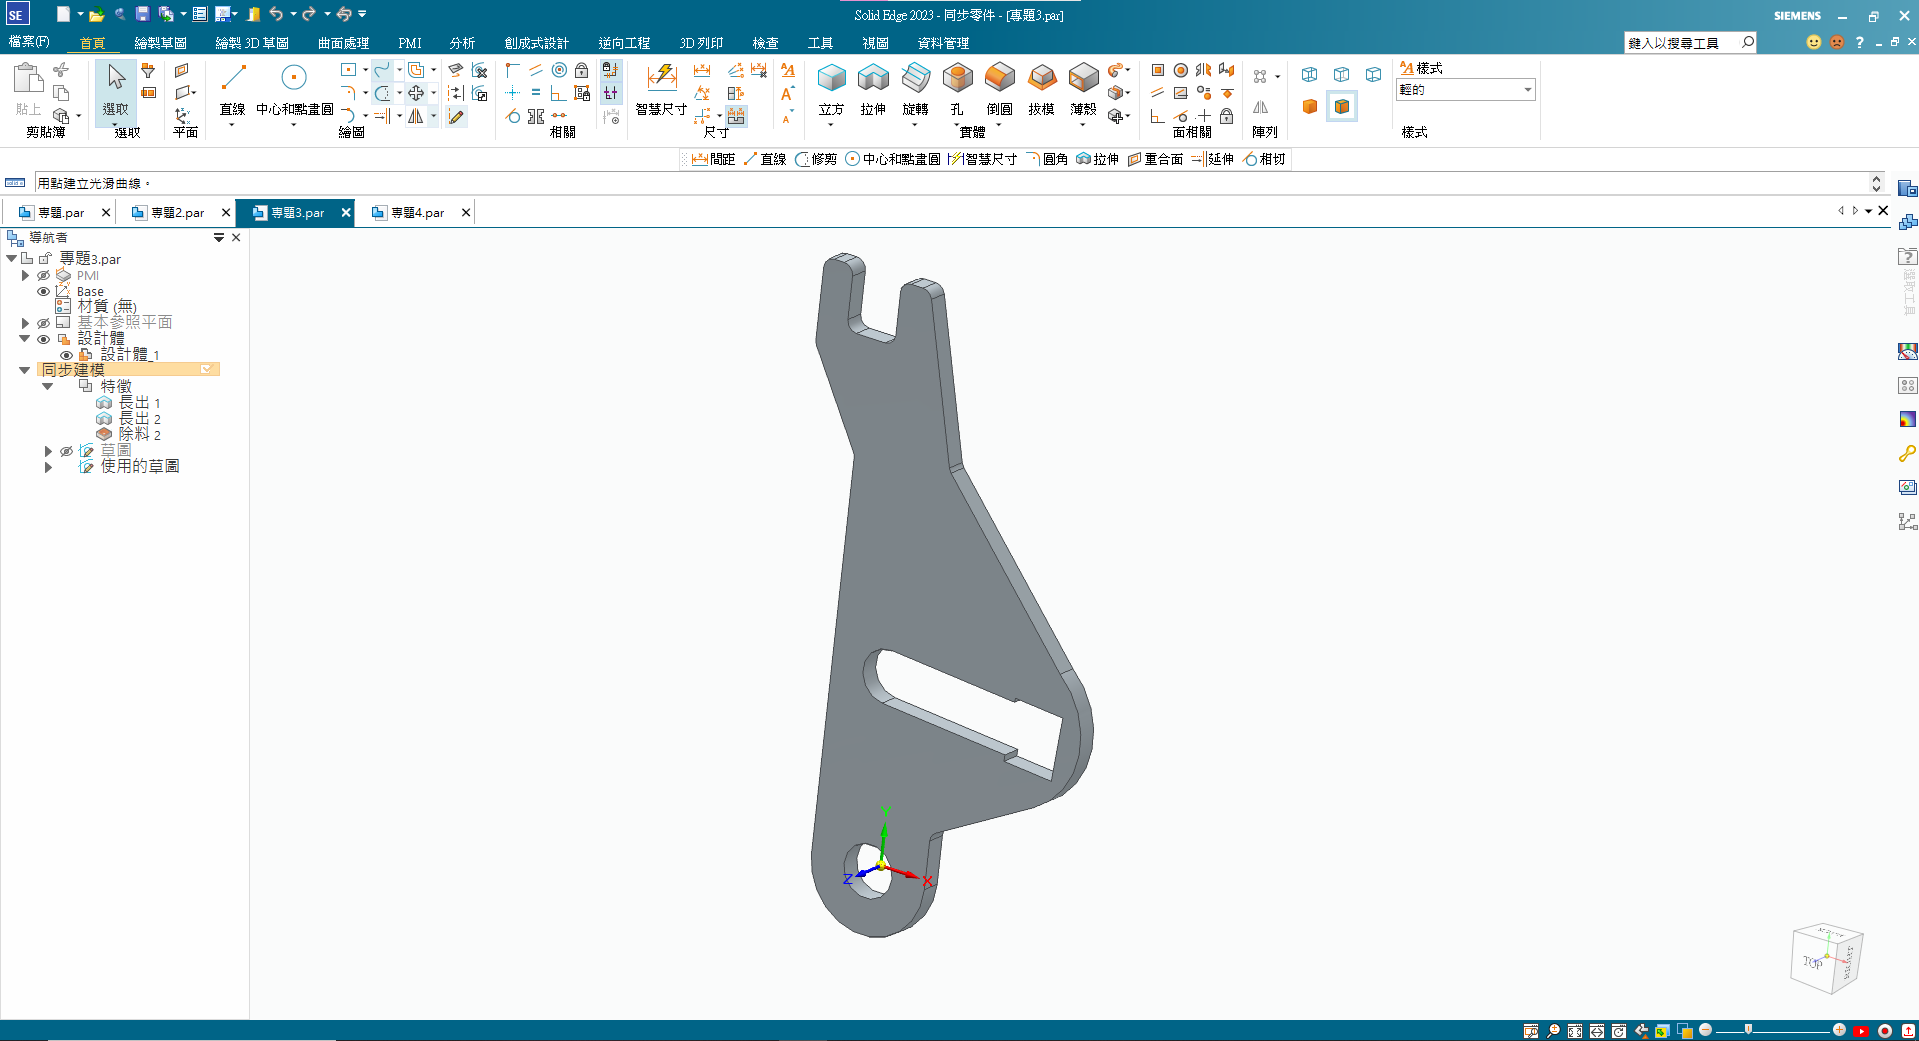
\includegraphics[width=10cm]{中控鎖3}
\caption{\Large 車門鎖零件模型}\label{4.8}
\end{center}
\end{figure}
\\
\begin{figure}[hbt!]
\begin{center}
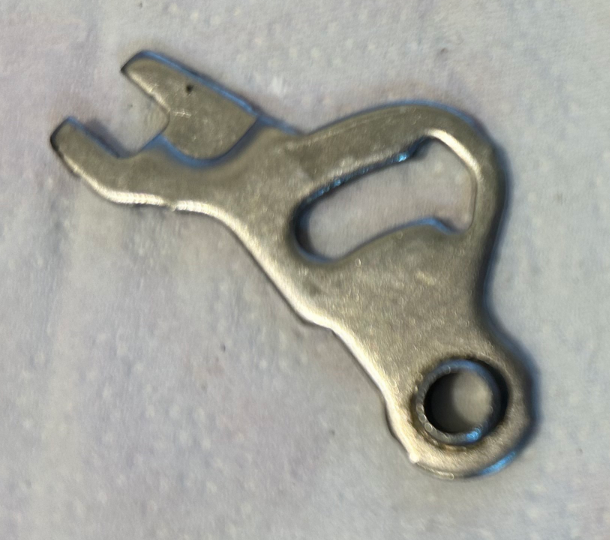
\includegraphics[width=10cm]{現實中控鎖4}
\caption{\Large 車門鎖結構零件}\label{4.4}
\end{center}
\end{figure}
\\
\begin{figure}[hbt!]
\begin{center}
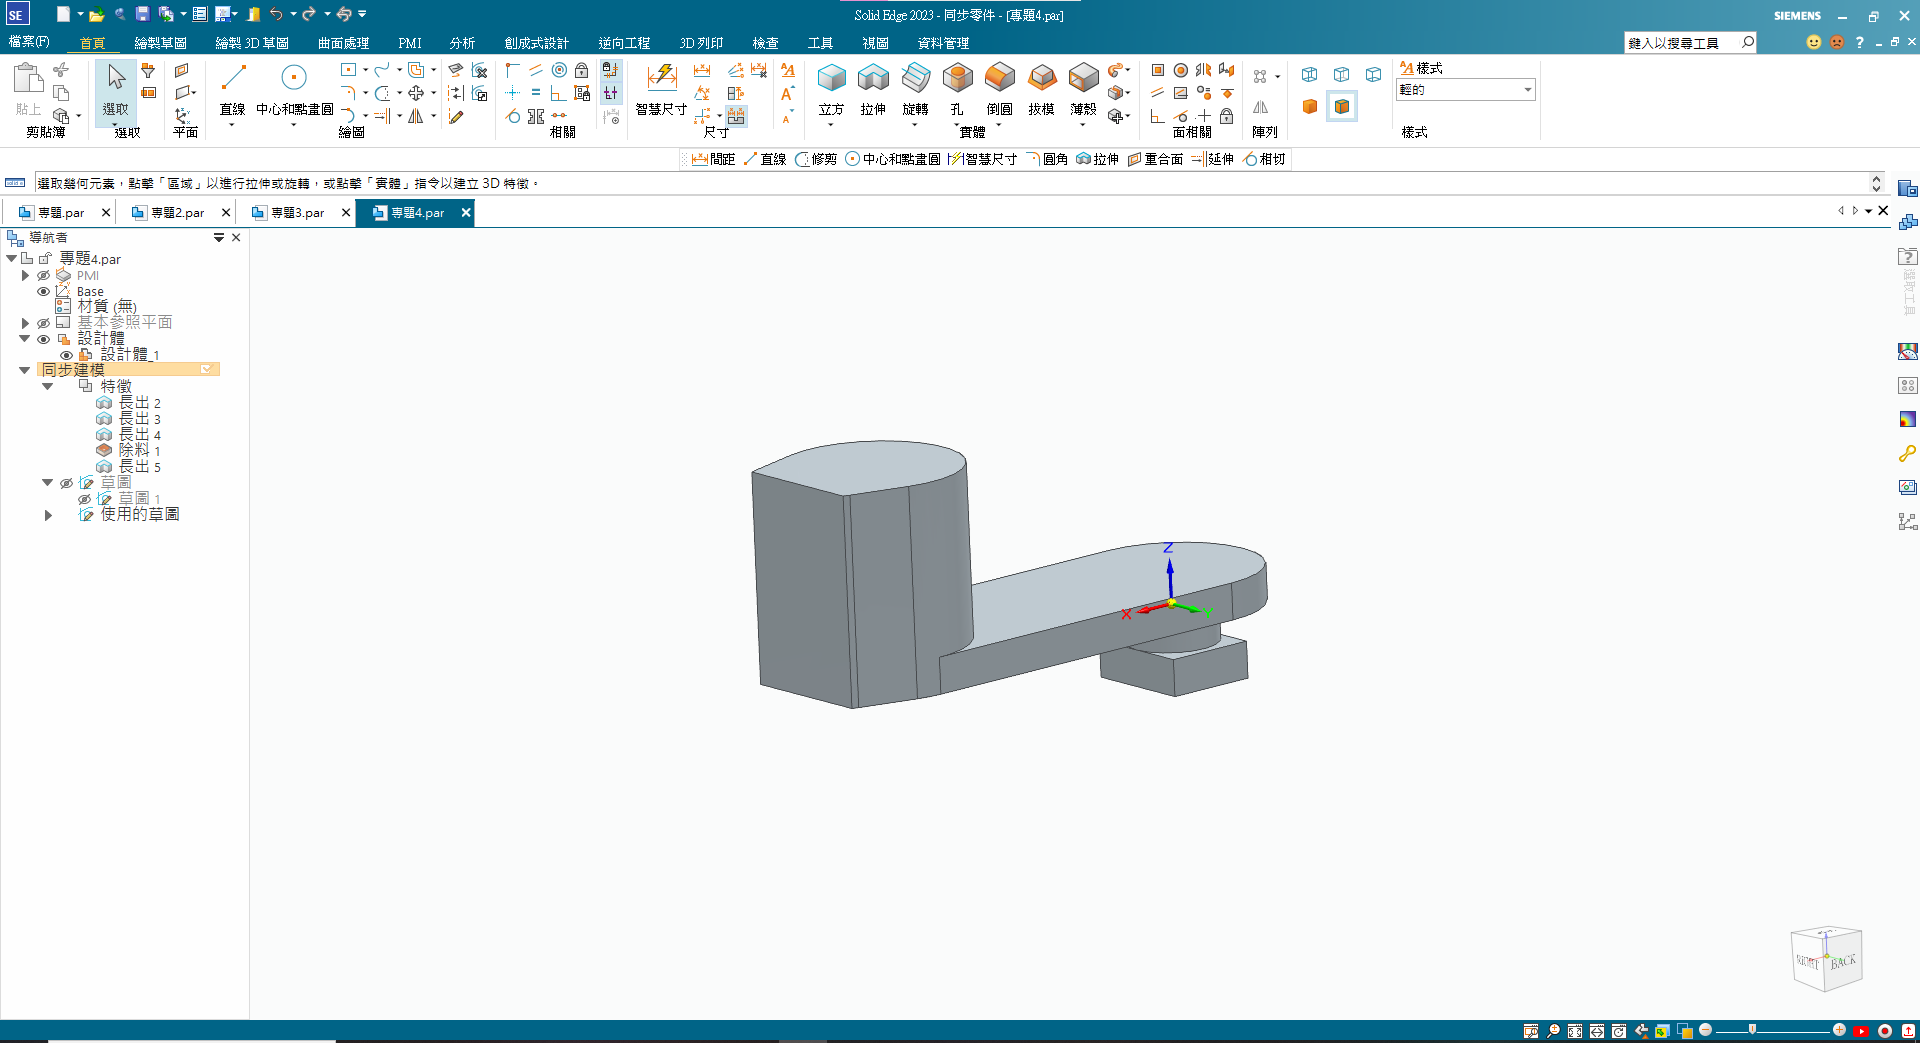
\includegraphics[width=10cm]{中控鎖4}
\caption{\Large 車門鎖零件模型}\label{4.9}
\end{center}
\end{figure}
\\
\begin{figure}[hbt!]
\begin{center}
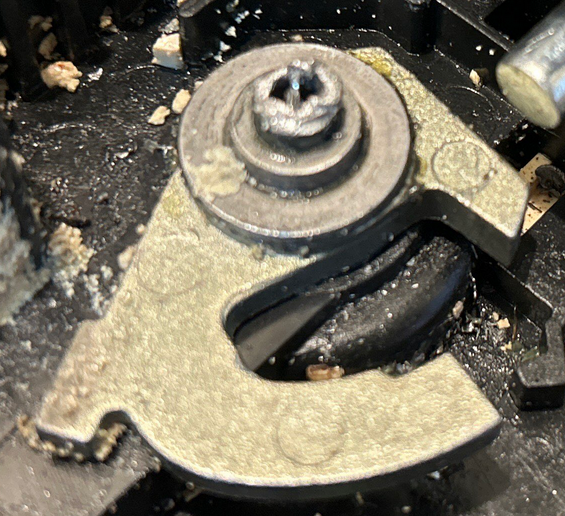
\includegraphics[width=10cm]{現實中控鎖5}
\caption{\Large 車門鎖結構}\label{4.5}
\end{center}
\end{figure}
\\
\begin{figure}[hbt!]
\begin{center}
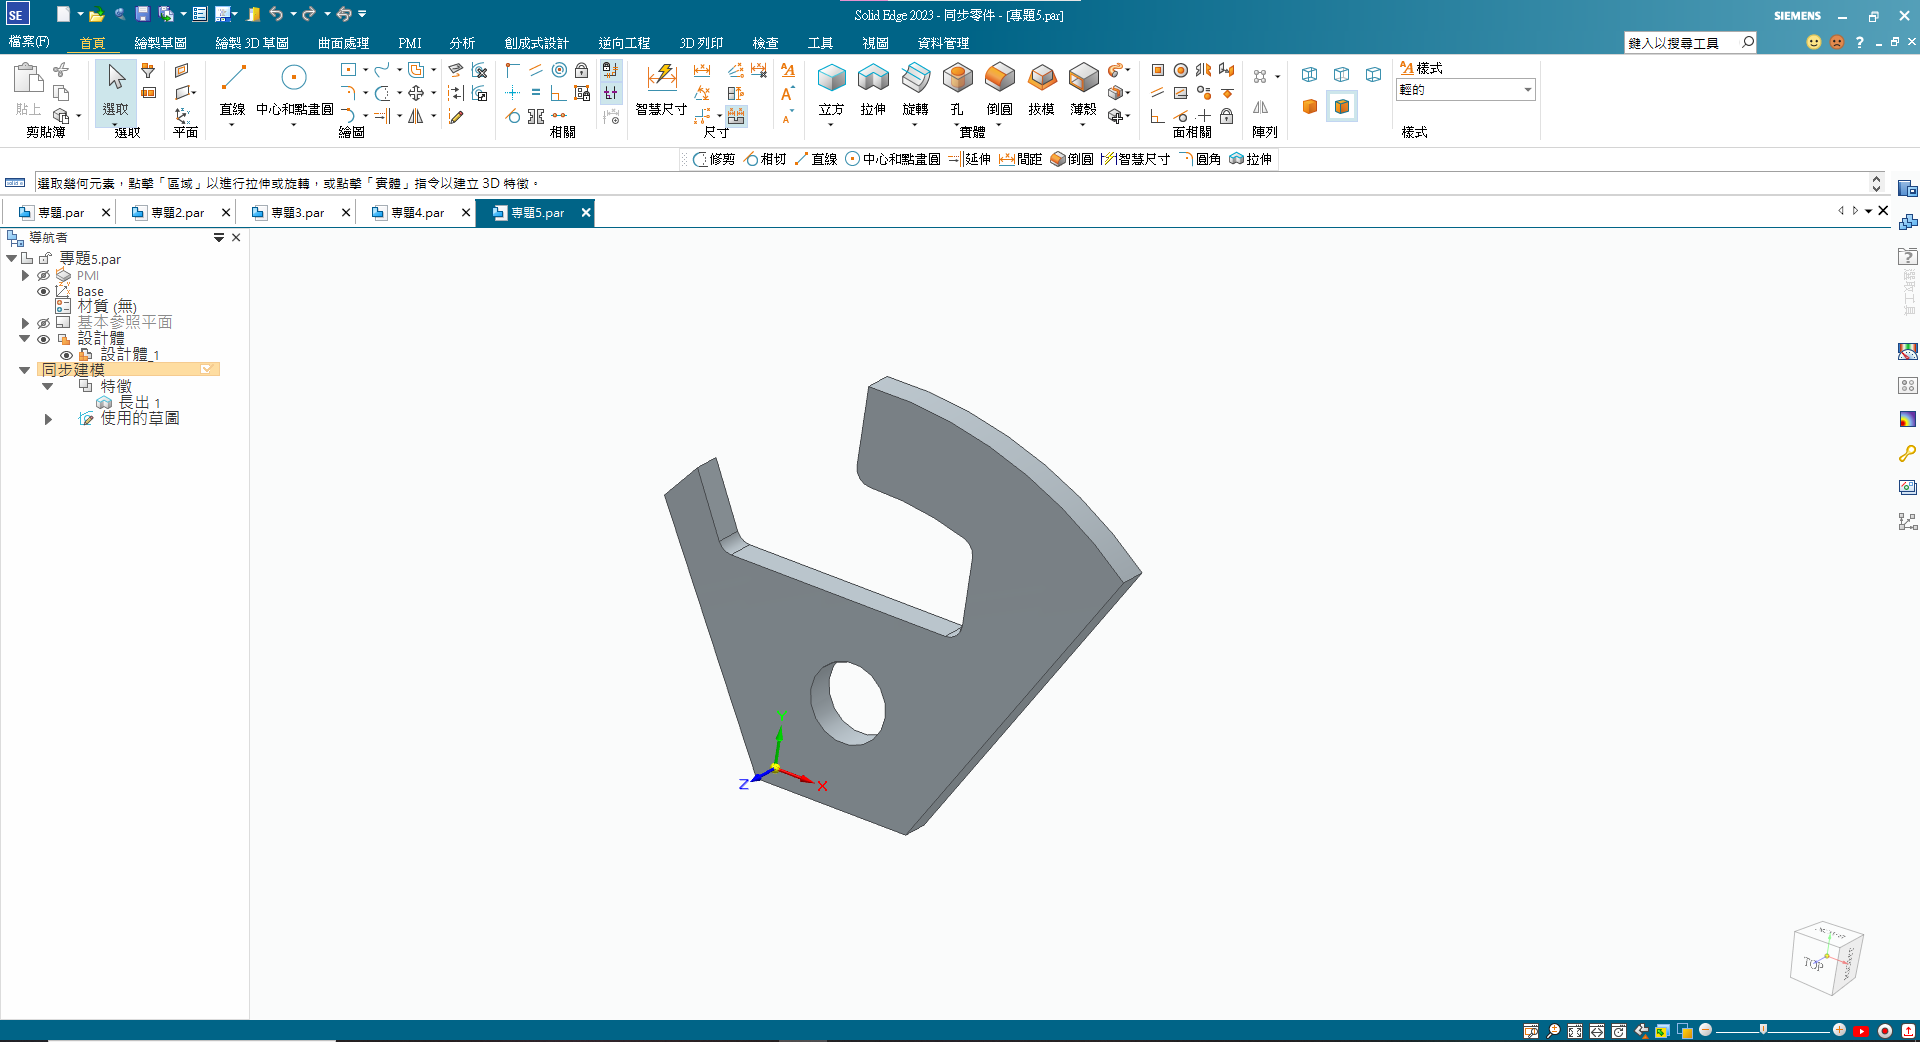
\includegraphics[width=10cm]{中控鎖5}
\caption{\Large 車門鎖零件模型}\label{4.10}
\end{center}
\end{figure}
\\

\newpage

\newpage

由圖\ref{4.11}所示,當我們要開內車門時,A件會往紅色軸方向轉動,帶動著B件與D件,讓C件朝粉色方向轉動達成開門的目的;開外車門時也是雷同,差別只在跳過A件,直接驅使B件作動。\\
\begin{figure}[hbt!]
\begin{center}
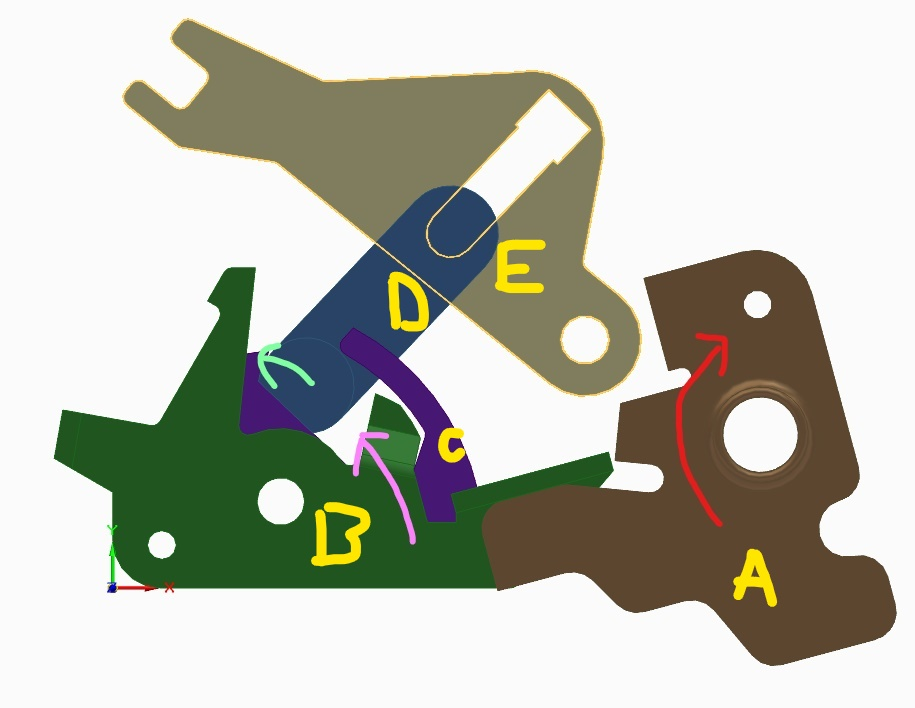
\includegraphics[width=10cm]{中控鎖組合圖2}
\caption{\Large 車門鎖零件模型}\label{4.11}
\end{center}
\end{figure}
\\

而當在我們把車鎖上門時,首先會使C件往橘色方向轉動,然後E件會向黑色方向轉動,帶動著D件向灰色方向移動,拖離運動區域,讓不管是開外車門還是內車門,B件都會式空轉狀態,如圖\ref{4.12}所示。\\
\begin{figure}[hbt!]
\begin{center}
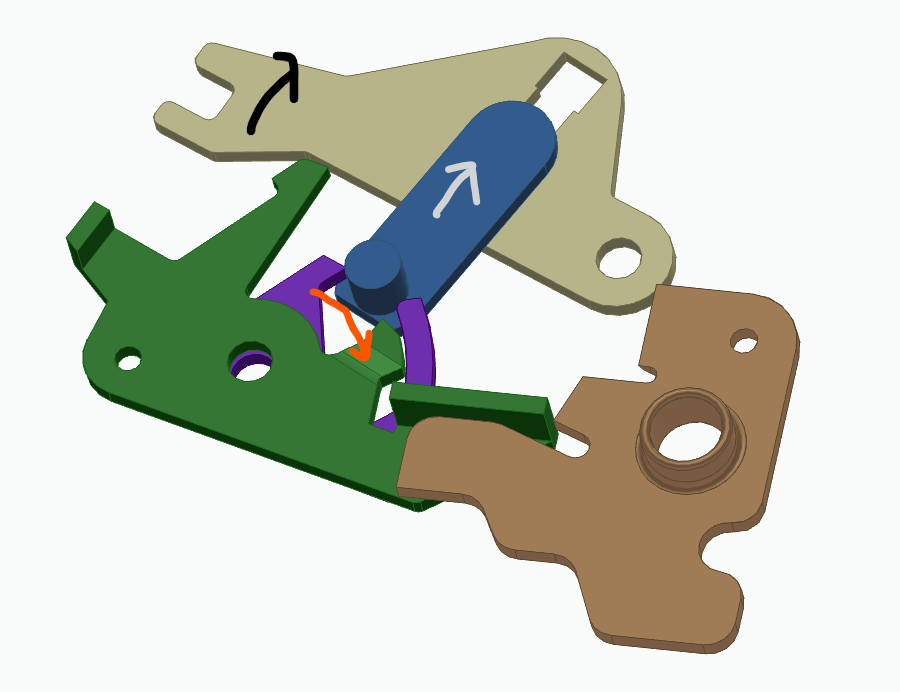
\includegraphics[width=10cm]{中控鎖組合圖3}
\caption{\Large 車門鎖零件模型}\label{4.12}
\end{center}
\end{figure}
\\

\newpage

\section{討論 Solid Edge 與 Femap 在機械設計課程應用的優勢}
在教學層面上來說,SolidWorks確實會比Solid Edge來的好教導,必進同步建模的關係,在3D圖修改尺寸的時候很有可能會因為沒設定好而改變其他零件的原始尺寸,而SolidWorks就算干擾到了其他特徵,有就只是Delete鍵按一按而已,但只是為了讓學生們學會繪圖軟體而已的話,那就已經失去教導的原始意義了,本身教育就是在[建立未來優勢]的前提下所產生的,對學生的未來來說,學Solid Edge會比學SolidWorks還來的有價值。\\

如果從高職開始學習Solid Edge,上了大學就會比學SolidWorks的學生來的有優勢,因為在學習Solid Edge的過程中,已經先了解了有限元素分析及生成式設計的功能,在上大學的課程之前,已經接觸過了在未來職場上會接觸到的東西,這對學生來說是非常有優勢的。\\

Solid Edge對學生上課來說,不用網路這個特點就非常的方便,有時候學校的使用人數過多,網路一斷,就連畫個圖都有困難了,而且家中也不可能買得起正版的SoildWorks能練習、作業,連線到學校的VPN也不是非常的方便,每次使用之前都必須先經過網路的連線才行,這導致很多學生都是使用非正版的軟體。而Solid Edge就沒這個問題,因為軟體不須透過網路來授權,所以就算斷線也不用害怕耽誤到作業的進度。\\

\newpage